

\Minisec{Kodierungen}
\begin{tabular}{|c|c|c|c|}
\hline
	& \textbf{0} & \textbf{1} & \textbf{Beispiel} \\
\hline
NRZ	& 	0		& 	1	& \includetablegraphics{0.25\textwidth}{NRZ}				\\
\hline
NRZI & 	 halten	&	 ändern	&	\includetablegraphics{0.25\textwidth}{NRZI}			\\
\hline
Manchester &  $0 \rightarrow 1$ &  $1 \rightarrow 0$& 	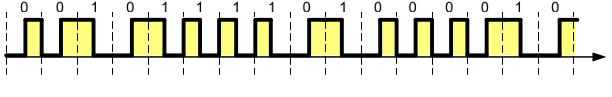
\includegraphics[width=0.25\textwidth]{Manchester}			\\
\hline
AMI 		& 0 & $\pm 1 $ & \ 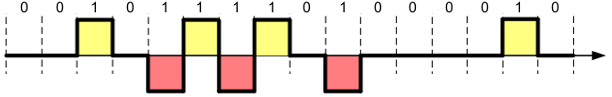
\includegraphics[width=0.25\textwidth]{AMI}	\\
\hline
\end{tabular}

\minisec{Code-Ersetzungen bei Ternären Codes (Rest wie bei AMI):}
\begin{tabular}{|c|c|c|}
\hline
Code:	& B8ZS &HDB3	\\
\hline
zu Ersetzen: & 8 Nullen	& 4	Nullen\\
\hline
Regel: 
&	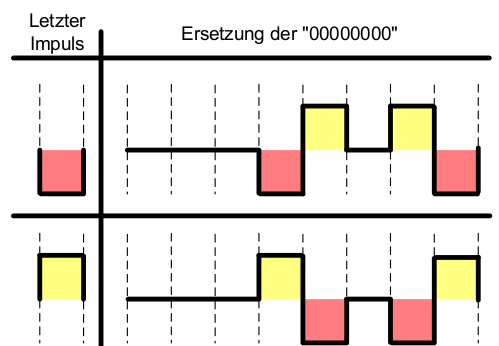
\includegraphics[width=0.2\textwidth]{B8ZS}		&	 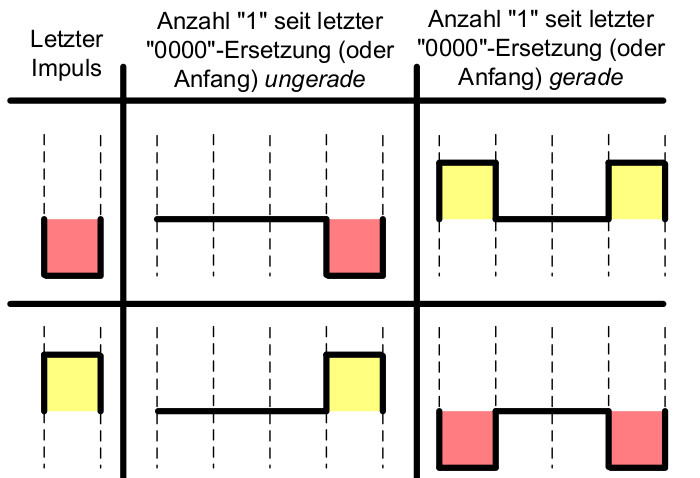
\includegraphics[width=0.2\textwidth]{HDB3} \\
\hline
\end{tabular}

\begin{minipage}{0.25\textwidth}
4B/5B mit maximal 3 Nullen in folge\\
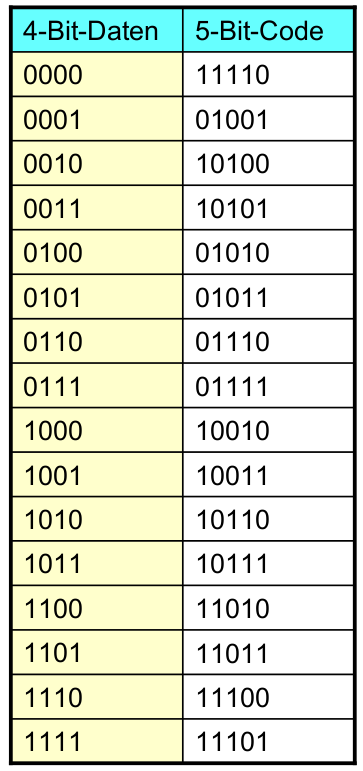
\includegraphics[angle=90 , width=\textwidth ]{4B5B}
\end{minipage}
\begin{minipage}{0.25\textwidth}
\centering
$ A = \log_2(B) \Leftrightarrow B = 2^A $
\end{minipage}

\newcommand{\formel}[1]{\fbox{$ #1 $}}
\newcommand{\tab}{\rule{0.5cm}{0pt}}

\Minisec{Übertragung}
\formel{v_{max} = 2 B;} \tab
\formel{D_{max} = 2 B \log_2(L)}\tab
\formel{D_{max} = B \log_2(1+ \frac{S}{N})}\tab
\formel{\frac{S}{N}= 10^{SNR[db]/10}}


$v_{max}$ = Schrittgeschwindigkeit; $D_{max}$ = Datenrate;	 B = Bandbreite; \\
L = Signalstufen; 	SNR = Signal-Rausch-Abstand [db]




